\section{System Model and Channel Generation}
\label{sec:system-model}


\begin{figure}[t]
  \centering
  \resizebox{0.95\columnwidth}{!}{% Urban Macrocell (UMa) System Model
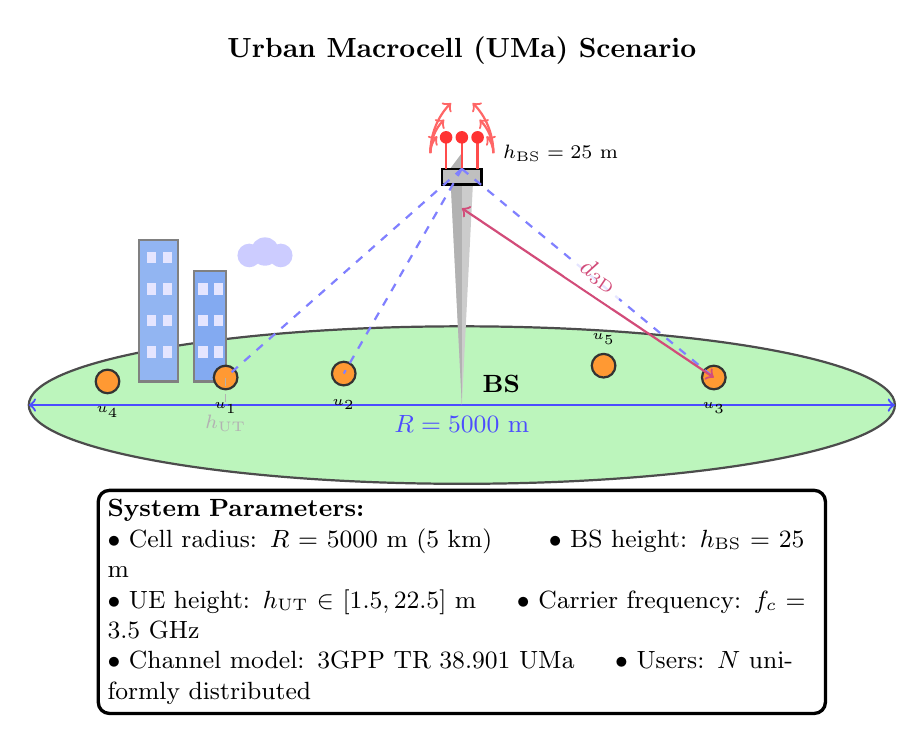
\begin{tikzpicture}[
    scale=1.0, every node/.style={scale=1.0}
]

% Define colors
\definecolor{skyblue}{RGB}{135,206,235}
\definecolor{groundgreen}{RGB}{144,238,144}
\definecolor{building}{RGB}{100,149,237}

% Ground circle (cell coverage)
\fill[groundgreen!60] (0,0) ellipse (5.5cm and 1cm);
\draw[thick, black!70] (0,0) ellipse (5.5cm and 1cm);

% Cell radius annotation
\draw[<->, thick, blue!70] (-5.5,-0) -- (5.5,-0) node[midway, below, font=\small] { $R = 5000$ m};

% Base Station Tower (CENTER)
\begin{scope}[xshift=0cm]
    % Tower structure
    \fill[gray!40] (0,0) -- (-0.15,3) -- (0.15,3) -- cycle;
    \fill[gray!60] (0,0) -- (-0.15,3) -- (0,3.2) -- cycle;
    
    % Platform at top
    \draw[fill=gray!50, thick] (-0.25,2.8) rectangle (0.25,3);
    
    % Antenna elements
    \foreach \x in {-0.2,0,0.2} {
        \draw[thick, red!70] (\x,3) -- (\x,3.4);
        \fill[red!80] (\x,3.4) circle (0.08);
    }
    
    % Signal waves
    \foreach \i in {1,2,3} {
        \draw[thick, red!60, ->] (-0.4,3.2) arc[start angle=180, end angle=135, radius=0.3*\i];
        \draw[thick, red!60, ->] (0.4,3.2) arc[start angle=0, end angle=45, radius=0.3*\i];
    }
    
    % BS label
    \node[font=\small\bfseries, below] at (0.5,0.5) {BS};
    \node[font=\scriptsize, right] at (0.4,3.2) {$h_{\mathrm{BS}} = 25$ m};
\end{scope}

% Buildings (left side)
\begin{scope}[xshift=-3.5cm, yshift=0.3cm]
    % Building 1
    \fill[building!70] (-0.6,0) rectangle (-0.1,1.8);
    \draw[thick, black!50] (-0.6,0) rectangle (-0.1,1.8);
    % Windows
    \foreach \y in {0.3,0.7,1.1,1.5} {
        \foreach \x in {-0.5,-0.3} {
            \fill[white!90!blue] (\x,\y) rectangle (\x+0.12,\y+0.15);
        }
    }
    
    % Building 2
    \fill[building!80] (0.1,0) rectangle (0.5,1.4);
    \draw[thick, black!50] (0.1,0) rectangle (0.5,1.4);
    % Windows
    \foreach \y in {0.3,0.7,1.1} {
        \foreach \x in {0.15,0.35} {
            \fill[white!90!blue] (\x,\y) rectangle (\x+0.12,\y+0.15);
        }
    }
    
    % Small cloud
    \fill[white!80!blue] (0.8,1.6) circle (0.15);
    \fill[white!80!blue] (1,1.65) circle (0.18);
    \fill[white!80!blue] (1.2,1.6) circle (0.15);
\end{scope}

% Users (UEs) distributed in cell
\begin{scope}
    % User 1 (near buildings, weak user)
    \fill[orange!80] (-3,0.35) circle (0.15);
    \draw[thick, black!80] (-3,0.35) circle (0.15);
    \node[font=\tiny, below] at (-3,0.15) {$u_1$};
    \draw[dashed, gray!60] (-3,0.35) -- (-3,0) node[below, font=\scriptsize] {$h_{\mathrm{UT}}$};
    
    % User 2 (middle-left)
    \fill[orange!80] (-1.5,0.4) circle (0.15);
    \draw[thick, black!80] (-1.5,0.4) circle (0.15);
    \node[font=\tiny, below] at (-1.5,0.2) {$u_2$};
    
    % User 3 (right, strong user) - for d3D annotation
    \fill[orange!80] (3.2,0.35) circle (0.15);
    \draw[thick, black!80] (3.2,0.35) circle (0.15);
    \node[font=\tiny, below] at (3.2,0.15) {$u_3$};
    
    % User 4 (far edge left)
    \fill[orange!80] (-4.5,0.3) circle (0.15);
    \draw[thick, black!80] (-4.5,0.3) circle (0.15);
    \node[font=\tiny, below] at (-4.5,0.1) {$u_4$};
    
    % User 5 (top right)
    \fill[orange!80] (1.8,0.5) circle (0.15);
    \draw[thick, black!80] (1.8,0.5) circle (0.15);
    \node[font=\tiny, above] at (1.8,0.65) {$u_5$};
\end{scope}

% Communication links (dashed lines from BS to users)
\draw[thick, dashed, blue!50] (0,3) -- (-3,0.35);
\draw[thick, dashed, blue!50] (0,3) -- (-1.5,0.4);
\draw[thick, dashed, blue!50] (0,3) -- (3.2,0.35);

% Distance annotations - d3D (3D distance from BS to user)
\draw[<->, thick, purple!70] (0,2.5) -- (3.2,0.35) node[midway, above, font=\small, sloped, fill=white, fill opacity=0.8, text opacity=1] {$d_{3\mathrm{D}}$};

% Title
\node[font=\normalsize\bfseries] at (0,4.5) {Urban Macrocell (UMa) Scenario};

% System parameters box
\node[draw, very thick, fill=white, rectangle, text width=90mm, font=\small, align=left, rounded corners] at (0,-2.5cm) {
\textbf{System Parameters:}\\
$\bullet$ Cell radius: $R = 5000$ m (5 km) \hspace{5mm} $\bullet$ BS height: $h_{\mathrm{BS}} = 25$ m\\
$\bullet$ UE height: $h_{\mathrm{UT}} \in [1.5, 22.5]$ m \hspace{3mm} $\bullet$ Carrier frequency: $f_c = 3.5$ GHz\\
$\bullet$ Channel model: 3GPP TR 38.901 UMa \hspace{3mm} $\bullet$ Users: $N$ uniformly distributed
};

\end{tikzpicture}
}
  \caption{Urban Macrocell (UMa) layout showing base station, distributed users, and 3GPP TR 38.901 channel model parameters.}
  \label{fig:3GPP Model}
\end{figure}

\subsection{Cell Layout and Notation}
We consider a single Urban Macro (UMa) cell of radius $R$ with a base station (BS) at height $h_{\mathrm{BS}}$, as illustrated in Fig.~\ref{fig:3GPP Model}. A total of $N$ users are uniformly dropped within the cell, where each user equipment (UE) has a height $h_{\mathrm{UT}}\in[1.5,22.5]$\,m. The carrier frequency is set to $f_c=3.5$\,GHz. On a single physical resource block (PRB), the BS transmits total power $P_{\mathrm{tot}}$ over bandwidth $B$, with noise power spectral density $N_0$ (so the noise power per PRB is $N_0B$). Let $h_u$ denote the complex channel coefficient for user $u$ and $|h_u|^2$ represent its channel power gain.

\subsection{3GPP TR 38.901 UMa Channel Model}
\label{subsec:38901}
We follow 3GPP TR~38.901 (UMa) for reproducible links \cite{etis2024}.

\paragraph*{LOS Probability}
Let $d_{2\mathrm{D}}$ be horizontal distance and $d_{3\mathrm{D}}$ the 3D distance. The UMa LOS probability is height-dependent per TR~38.901; we sample LOS/NLOS accordingly and condition subsequent large/small-scale models on that draw.

\paragraph*{Large-Scale Path Loss}
For frequency in GHz and $d_{3\mathrm{D}}$ in meters, representative UMa formulas are
\[
\mathrm{PL}_{\mathrm{LOS}}(d_{3\mathrm{D}})=28+22\log_{10}(d_{3\mathrm{D}})+20\log_{10}\!\Big(\tfrac{f_c}{1\,\mathrm{GHz}}\Big)\ \mathrm{dB},
\]
\[
\mathrm{PL}_{\mathrm{NLOS}}(d_{3\mathrm{D}},h_{\mathrm{UT}})=13.54+39.08\log_{10}(d_{3\mathrm{D}})
+20\log_{10}\!\Big(\tfrac{f_c}{1\,\mathrm{GHz}}\Big)-0.6(h_{\mathrm{UT}}-1.5)\ \mathrm{dB}.
\]
Lognormal shadowing $X_\sigma\sim\mathcal{N}(0,\sigma^2)$ (in dB) is applied. The large-scale power gain is
\[
g_{\mathrm{LS}}=10^{-(\mathrm{PL}+X_\sigma)/10}.
\]

\paragraph*{Small-Scale Fading}
LOS links use Rician fading (e.g., $K\!\approx\!9$\,dB); NLOS links use Rayleigh. The composite channel magnitude obeys
\[
|h_u| \;=\; \sqrt{g_{\mathrm{LS}}}\;\sqrt{g_{\mathrm{SS}}},\quad |h_u|^2 = g_{\mathrm{LS}}\,g_{\mathrm{SS}}.
\]

\subsection{PD-NOMA SINR, SIC, and Rates}
Consider a NOMA pair $(i,j)$ on one PRB. Without loss of generality, let $i$ be the \emph{weak} user ($|h_i|<|h_j|$) and $j$ the \emph{strong} user. Allocate a power split
\[
P_i = \alpha P_{\mathrm{tot}},\qquad P_j = (1-\alpha)P_{\mathrm{tot}},\qquad \alpha\in(0,1),
\]
with the weak user typically receiving \emph{more} power (i.e., $\alpha>0.5$).

\paragraph*{Receiver SINRs}
The weak user treats the strong user as interference:
\[
\mathrm{SINR}_i(\alpha)=\frac{\alpha P_{\mathrm{tot}}|h_i|^2}{(1-\alpha)P_{\mathrm{tot}}|h_i|^2 + N_0 B}.
\]
The strong user first decodes $i$ (for SIC):
\[
\mathrm{SINR}_{j\leftarrow i}(\alpha)=\frac{\alpha P_{\mathrm{tot}}|h_j|^2}{(1-\alpha)P_{\mathrm{tot}}|h_j|^2 + N_0 B}.
\]
After cancelling $i$, the strong user decodes itself interference-free:
\[
\mathrm{SINR}_j(\alpha)=\frac{(1-\alpha)P_{\mathrm{tot}}|h_j|^2}{N_0 B}.
\]

\paragraph*{SIC Feasibility and Guard}
Let $\Gamma_i$ be the SNR (linear) required to support $i$’s target rate on the PRB, and let $\Delta_{\min}$ be a practical SIC margin (in dB). SIC is feasible if
\[
10\log_{10}\!\big(1+\mathrm{SINR}_{j\leftarrow i}(\alpha)\big) \;\ge\; 10\log_{10}(1+\Gamma_i) + \Delta_{\min}.
\]
A simple pre-screen also helps: a channel disparity guard
\[
10\log_{10}\!\Big(\frac{|h_j|^2}{|h_i|^2}\Big)\ \ge\ \Gamma_{\mathrm{SIC}}\ \text{(dB)},
\]
with $\Gamma_{\mathrm{SIC}}$ chosen from implementation limits.

\paragraph*{Per-PRB Rates and Sum-Rate}
For a given $\alpha$,
\[
R_i(\alpha)=\log_2\!\big(1+\mathrm{SINR}_i(\alpha)\big),\quad
R_j(\alpha)=\log_2\!\big(1+\mathrm{SINR}_j(\alpha)\big),
\]
\[
R_{\mathrm{sum}}(\alpha)=R_i(\alpha)+R_j(\alpha).
\]
Edge weights for matching (Sec.~\ref{sec:graph-matching}) often use
\[
w_{ij}\;=\;\max_{\alpha\in(0,1)}\ R_{\mathrm{sum}}(\alpha)\quad
\text{subject to SIC feasibility and $\alpha_{\min}\le\alpha\le\alpha_{\max}$.}
\]
A reasonable baseline power split is to bias power toward the weaker channel, e.g.,
\[
\alpha \;=\; \frac{|h_j|^{-\beta}}{|h_i|^{-\beta}+|h_j|^{-\beta}},\quad \beta\!\in\![1,2],
\]
which increases $\alpha$ as $|h_i|$ weakens (set $\beta\!=\!1$ for inverse-gain weighting).

\subsection{Channel and Geometry Visualizations}
\label{subsec:channel-geometry}

\vspace{2mm} % small spacing under subsection title

\begin{figure}[t]
  \centering
  
\includegraphics[width=0.9\linewidth]{user_distribution.png}
  \vspace{-2mm}
  \caption{User distribution within the cell, colored by channel gain (dB).}
  \label{fig:user_distribution}
  \vspace{-1mm}
\end{figure}

\begin{figure}[t]
  \centering
  
\includegraphics[width=0.9\linewidth]{channel_characteristics.png}
  \vspace{-2mm}
  \caption{Channel characteristics: (top-left) channel-gain histogram, (top-right) path-loss vs.\ distance, (bottom-left) fading distribution, (bottom-right) sorted gains.}
  \label{fig:channel_characteristics}
  \vspace{-1mm}
\end{figure}

\begin{figure}[t]
  \centering
  
\includegraphics[width=0.9\linewidth]{channel_components_analysis.png}
  \vspace{-2mm}
  \caption{Decomposition of channel components (path loss, shadowing, fading) and distance–gain scatter with summary statistics.}
  \label{fig:channel_components}
  \vspace{-1mm}
\end{figure}

\begin{figure}[t]
  \centering
  
\includegraphics[width=0.9\linewidth]{user_positioning_analysis.png}
  \vspace{-2mm}
  \caption{Radial and angular user distribution: polar view (colored by gain) and angle–distance map.}
  \label{fig:user_positioning}
  \vspace{-2mm}
\end{figure}

Figures~\ref{fig:user_distribution}–\ref{fig:user_positioning} present a comprehensive visualization of the simulated 3GPP~TR~38.901 Urban Macro (UMa) channel environment generated for $N=500$ users uniformly distributed within a $5$\,km cell. 
Figure~\ref{fig:user_distribution} shows the spatial user distribution across the cell, with color representing the overall channel gain in dB. Users closer to the base station exhibit higher channel gains, while those near the cell edge experience significant attenuation, confirming the expected radial decay in power. 
Figure~\ref{fig:channel_characteristics} illustrates the statistical characteristics of the channel components: the top-left histogram shows the channel-gain distribution, the top-right plot presents the path-loss variation with distance, the bottom-left histogram displays the Rayleigh fading distribution for NLOS users, and the bottom-right subplot depicts the sorted channel-gain curve highlighting user diversity. 
Figure~\ref{fig:channel_components} further decomposes the composite channel into its constituent effects—path loss, shadowing, and small-scale fading—through scatter and box plots, providing insight into their relative contributions and the statistical variability of each. 
Finally, Figure~\ref{fig:user_positioning} analyzes the user positioning geometry: the polar plot and angle–distance scatter demonstrate uniform azimuthal distribution, while the radial and angular histograms confirm homogeneous spatial deployment. Collectively, these figures validate the correctness of the 3GPP-compliant CSI generation procedure and provide a clear foundation for subsequent NOMA pairing and clustering analysis.
